\chapter{Arhitektura i dizajn sustava}
		
		Arhitektura sustava može se podijelit na tri glavna podsustava: web preglednik, web poslužitelj i baza podataka.
	\begin{itemize}
		\item 	\textbf{Web preglednik} – program koji služi za pristupanje web stranicama. Putem web preglednika korisnik komunicira sa poslužiteljem koristeći princip zahtjev-odgovor ili šalje podatke (najčešće u obliku obrazaca). Daljnja zadaća web preglednika je osigurati da se traženi podaci ispravno prikazuju ili da se ispravno prosljeđuju i spremaju na poslužitelj.
		\item 	\textbf{Web poslužitelj} – glavni je dio web aplikacije. To je most koji povezuje korisnika i bazu podataka koji se temelji na protokolu HTTP. Na zahtjeve korisnika dohvaća tražene podatke (resurse) ili obrađuje i sprema poslane podatke od korisnika.
		\item 	\textbf{Baza podataka} – srce je sustava. U njoj su pospremljeni svi podaci. Skoro ne postoji sustav u kojem nema komunikacije između aplikacije i baze.	
	\end{itemize}
		Aplikacije je izgrađena na modelu MVC (Model – View - Controller) softverske arhitekture uz male modifikacije. Controller dio strukture je ostvaren tako što je integriran unutar same baze, tj. funkcije koje manipuliraju podacima se nalaze unutar baze. Shodno tome aplikaciju onda dijelimo na tri komponente:
	\begin{itemize}
		\item	\textbf{Model} – glavna komponenta sustava. Reprezentira strukturu podataka.
		\item	\textbf{View} – komponenta zaslužna za reprezentaciju podataka.
		\item	\textbf{Controller} – komponenta koja odrađuje svu logiku i komunikaciju između sučelja i baze.
	\end{itemize}
	
		\smallskip
		Backend naše aplikacije je ostvaren direktno u bazi postgreSQL(razvojno sučelje pgadmin) za što koristimo API napisan u Node.js frameworku Express, koji služi kao middleware. Za izradu frontend-a korišten je React uz pomoć Material UI. Razvojno okruženje koje smo koristili je bilo Visual Studio Code.
		

		

				
		\section{Baza podataka}
			
			%\textbf{\textit{dio 1. revizije}}\\
			
		%\textit{Potrebno je opisati koju vrstu i implementaciju baze podataka ste odabrali, glavne komponente od kojih se sastoji i slično.}
			U ovom projektu koristit ćemo relacijsku bazu podataka, čije su osnovne jedinke entiteti, definirani imenom i skupom atributa. Osnovna zadaća baze podataka je pohrana podataka te brza i efikasna obrada tih podataka u ovisnosti i korisničkim zahtjevima. U bazi podataka su pohranjeni podaci o korisnicima, njihovim ulogama, preferencijama, kao i o smještaju te dostupnosti smještaja. Dodatno uz navedeno, zbog zahtjeva organizacije prijevoza, baza također sprema informacije o vrstama vozila i dostupnosti tih vozila kao i o vremenu i mjestu boravka korisnika zdravstvenog turizma. Tako su i definirani sljedeći entiteti:
			\begin{multicols}{2}
				\begin{itemize}
					\item Accommodation
					\item AccommodationOccupied
					\item AccommodationType
					\item AdminUser
					\item Assigned
					\item AssignedRole
					\item Clinic
					\item Credentials
					\item Equipped
					\item Patient
					\item PatientArrival
					\item PatientPlan
					\item PatientPreferences
					\item Town
					\item Transporter
					\item Treatment
					\item UserRole
					\item Vehicle
					\item VehicleOccupied
					\item VehicleSchedule
					\item VehicleType
				\end{itemize}
			\end{multicols}
		
			\subsection{Opis tablica}
			
				%Accommodation
				\textbf{Accommodation} Ovaj entitet sadrži podatke o smještaju, vrsti smještaja, njegovoj opremljenosti te adresi na kojoj se nalazi kao i koordinatama. Atributi su: AccommodationID (primary key), realEstateID, TypeID (foreign key), EquippedID (foreing key), latitude, longitude, address, TownID (foreign key), ClinicID (foreign key), active. Ovaj je entitet u vezi Many-to-One sa entitetom Town preko atributa TownID,u vezi Many-to-One sa entitetom Clinic preko atributa TownID, nadalje u vezi Many-to-One sa entitetom AccommodationType preko atributa TypeID, u vezi Many-to-One sa entitetom Equipped preko atributa EquippedID, u vezi One-to-One sa entitetom Patient preko atributa AccommodationID i PatientID.
				
				\begin{longtblr}[
					label=none,
					entry=none
					]{
						width = \textwidth,
						colspec={|X[10,l]|X[6, l]|X[20, l]|}, 
						rowhead = 1,
					} %definicija širine tablice, širine stupaca, poravnanje i broja redaka naslova tablice
					\hline \SetCell[c=3]{c}{\textbf{Accommodation}}	 \\ \hline[3pt]
					\SetCell{LightGreen}AccommodationID & BIGSERIAL & Jedinstveni brojčani identifikator smještaja, automatski generiran \\ \hline
					realEstateID & VARCHAR & Jedinstveni kod smještaja \\ \hline
					\SetCell{LightBlue} TypeID & INT & ID vrste smještaja \\ \hline
					\SetCell{LightBlue} EquippedID & INT & ID opremljenosti smještaja \\ \hline
					latitude & DECIMAL & Geografska širina  \\ \hline 
					longitude & DECIMAL & Geografska dužina	\\ \hline 
					address & VARCHAR & Adresa smještaja	\\ \hline
					\SetCell{LightBlue} TownID & INT & ID grada u kojem se smještaj nalazi \\ \hline
					\SetCell{LightBlue} ClinicID & INT & ID klinike kojoj smještaj pripada \\ \hline
					active & BIT & Je li smještaj upotrebljiv \\ \hline
				\end{longtblr}
				
				%AccommodationOccupied
				\textbf{AccommodationOccupied} Ovaj entitet sadrži podatke o zauzetosti smještaja kojima raspolaže pojedina klinika. Atributi su: PatientID (foreign key), AccommodationID (foreign key), dateTo, dateFrom. Ovaj je entitet u One-to-One vezi sa entitetom Accommodation preko atributa AccommodationID te u One-to-One vezi sa entiteom Patient preko atributa PatientID.
				
				\begin{longtblr}[
					label=none,
					entry=none
					]{
						width = \textwidth,
						colspec={|X[10,l]|X[6, l]|X[20, l]|}, 
						rowhead = 1,
					} %definicija širine tablice, širine stupaca, poravnanje i broja redaka naslova tablice
					\hline \SetCell[c=3]{c}{\textbf{AccommodationOccupied}}	 \\ \hline[3pt]
					\SetCell{LightGreen}occupationID & BIGSERIAL & Jedinstveni identifikator rekorda zauzeća smještaja \\ \hline
					\SetCell{LightBlue}PatientID & BIGSERIAL & Jedinstveni identifikator pacijenta \\ \hline
					\SetCell{LightBlue}AccommodationID & BIGSERIAL & Jedinstveni identifikator smještaja \\ \hline
					dateFrom & DATE & Datum od kojeg je smještaj dostupan \\ \hline
					dateTo & DATE & Datum do kojeg je smještaj dostupan \\ \hline 
				\end{longtblr}
				
				\break
				
				%AccommodationType
				\textbf{AccommodationType} Ovaj entitet sadrži podatke o tipu smještaja (stan u zgradi, stan u kući, iznajmljeno, u vlasništvu klinike). Atributi su: TypeID (primary key), description. Ovaj je entitet u One-to-Many vezi s entitetom Accommodation preko atributa TypeID.
				
				\begin{longtblr}[
					label=none,
					entry=none
					]{
						width = \textwidth,
						colspec={|X[8,l]|X[6, l]|X[20, l]|}, 
						rowhead = 1,
					} %definicija širine tablice, širine stupaca, poravnanje i broja redaka naslova tablice
					\hline \SetCell[c=3]{c}{\textbf{AccommodationType}}	 \\ \hline[3pt]
					\SetCell{LightGreen}TypeID & SMALLINT & Jedinstveni identifikator vrste smještaja, automatski generiran \\ \hline
					description & TEXT & Opis vrste smještaja (stan u kući, stan u zgradi, soba u hotelu ili motelu)	\\ \hline 
				\end{longtblr}
				
				%AdminUser
				\textbf{AdminUser} Ovaj entitet sadrži podatke o korisnicima aplikacije; svi administratori i oni koji mogu dodavati ili ažurirati ili brisati podatke iz baze. Atributi su: UserID (primary key), PIN(personal identification number), firstname, lastname, phone, email. Ovaj je entitet u vezi Many-to-Many sa entitetom UserRole preko atributa RoleID te u vezi One-to-One sa entitetom Credentials preko atributa UserID.
				
				\begin{longtblr}[
					label=none,
					entry=none
					]{
						width = \textwidth,
						colspec={|X[8,l]|X[6, l]|X[20, l]|}, 
						rowhead = 1,
					} %definicija širine tablice, širine stupaca, poravnanje i broja redaka naslova tablice
					\hline \SetCell[c=3]{c}{\textbf{AdminUser}}	 \\ \hline[3pt]
					\SetCell{LightGreen}UserID & BIGSERIAL & Jedinstveni brojčani identifikator korisnika, automatski generiran \\ \hline
					PIN & INT & Identifikacijski broj korisnika	\\ \hline 
					firstname & VARCHAR & Ime korisnika  \\ \hline 
					lastname & VARCHAR & Prezime korisnika	\\ \hline 
					phone & VARCHAR & Broj mobitela korisnika \\ \hline
					email & VARCHAR & Elektronička pošta korisnika \\ \hline
				\end{longtblr}
				
				\break
				
				%Assigned
				\textbf{Assigned} Ovaj entitet sadrži podatke o pridjeljenim tretmanima pacijentima te datum od kada to kada je koji pacijent na kojem tretmanu.Atributi su: TreatmentID (foreign key), PatientID (foreign key), dot. Ovaj je entitet u vezi One-to-Many sa entitetom Patient preko atributa PatientID te u vezi One-to-Many sa entitetom Treatment preko atributa TreatmentID.
				
				\begin{longtblr}[
					label=none,
					entry=none
					]{
						width = \textwidth,
						colspec={|X[8,l]|X[6, l]|X[20, l]|}, 
						rowhead = 1,
					} %definicija širine tablice, širine stupaca, poravnanje i broja redaka naslova tablice
					\hline \SetCell[c=3]{c}{\textbf{Assigned}}	 \\ \hline[3pt]
					\SetCell{LightBlue}TreatmentID & BIGSERIAL & Jedinstveni identifikator tretmana \\ \hline
					\SetCell{LightBlue}PatientID & BIGSERIAL & Jedinstveni identifikator pacijenta \\ \hline
					dot & DATE & Datum tretmana \\ \hline
				\end{longtblr}
				
				%AssignedRole
				\textbf{AssignedRole} Ovaj entitet sadrži podatke o pridjeljenim ulogama administratora. Atributi su: UserID (foreign key), RoleID (foreign key). Ovaj je entitet u vezi One-to-Many sa entitetom AdminUser preko atributa UserID te u vezi One-to-Many sa entitetom UserRole preko atributa RoleID.
				
				\begin{longtblr}[
					label=none,
					entry=none
					]{
						width = \textwidth,
						colspec={|X[8,l]|X[6, l]|X[20, l]|}, 
						rowhead = 1,
					} %definicija širine tablice, širine stupaca, poravnanje i broja redaka naslova tablice
					\hline \SetCell[c=3]{c}{\textbf{AssignedRole}}	 \\ \hline[3pt]
					\SetCell{LightBlue}UserID & BIGSERIAL & Jedinstveni identifikator adminstratora \\ \hline
					\SetCell{LightBlue}RoleID & BIGSERIAL & Jedinstveni identifikator uloge \\ \hline
				\end{longtblr}

				\break

				%Clinic
				\textbf{Clinic} Ovaj entitet sadrži podatke o klinikama u odabranoj zemlji. Atributi su: ClinicID (primary key), clinicName, latitude, longitude, clinicAddress, TownID (foreign key). Ovaj je entitet u vezi Many-to-One sa entitetom Town preko atributa TownID, u Many-to-Many vazi sa entitetom Accommodation preko atributa AccommodationID i ClinicID, u Many-to-Many vezi sa entitetom Transporter preko atributa TransporterID i ClinicID , u One-to-Many vezi sa entitetom PatientPlan preko atributa PatientID i ClinicID te u Many-to-Many vezi sa entitetom Treatment preko atributa TreatmentID.
				
				\begin{longtblr}[
					label=none,
					entry=none
					]{
						width = \textwidth,
						colspec={|X[8,l]|X[6, l]|X[20, l]|}, 
						rowhead = 1,
					} %definicija širine tablice, širine stupaca, poravnanje i broja redaka naslova tablice
					\hline \SetCell[c=3]{c}{\textbf{Clinic}}	 \\ \hline[3pt]
					\SetCell{LightGreen}ClinicID & BIGSERIAL & Jedinstveni brojčani identifikator klinike,automatski generiran \\ \hline
					clinicName & VARCHAR & Ime klinike	\\ \hline  
					Latitude & DECIMAL	& Geografska širina	\\ \hline 
					Longitude & DECIMAL & Geografska dužina \\ \hline
					clinicAddress & VARCHAR & Adresa klinike  \\ \hline
					\SetCell{LightBlue}TownID & INT & Grad u kojem se klinika nalazi \\ \hline
				\end{longtblr}
				
				%Credentials
				\textbf{Credentials} Ovaj entitet sadrži podatke o korisničkim računima administratora. Atributi su: UserID (foreign key), username i pass. Ovaj je entitet u One-to-One vezi sa entitetom AdminUser preko atributa UserID.
				
				\begin{longtblr}[
					label=none,
					entry=none
					]{
						width = \textwidth,
						colspec={|X[8,l]|X[6, l]|X[20, l]|}, 
						rowhead = 1,
					} %definicija širine tablice, širine stupaca, poravnanje i broja redaka naslova tablice
					\hline \SetCell[c=3]{c}{\textbf{Credentials}}	 \\ \hline[3pt]
					\SetCell{LightBlue}UserID & BIGSERIAL & ID korisnika kojem pripadaju korisničko ime i lozinka \\ \hline
					username & VARCHAR & Jedinstveno korisničko ime \\ \hline
					pass & VARCHAR & Lozinka korisnika za prijavu u aplikaciju	\\ \hline 
				\end{longtblr}
				
				\break
				
				%Equipped
				\textbf{Equipped} Ovaj entitet sadrži podatke o vrsti opremljenosti smještaja (potpuno opremljen, djelomično opremljen). Atributi su: EquippedID (primary key), description. Ovaj je entitet u One-to-Many vezi sa entitetom Accommodation preko atributa EquippedID.
				
				\begin{longtblr}[
					label=none,
					entry=none
					]{
						width = \textwidth,
						colspec={|X[8,l]|X[6, l]|X[20, l]|}, 
						rowhead = 1,
					} %definicija širine tablice, širine stupaca, poravnanje i broja redaka naslova tablice
					\hline \SetCell[c=3]{c}{\textbf{Equipped}}	 \\ \hline[3pt]
					\SetCell{LightGreen}EquippedID & SMALLINT & Jedinstveni identifikator opremljenosti smještaja, automatski generiran \\ \hline
					description & TEXT & Opis opremljenosti smještaja (potpuno opremljen, djelomično opremljen)	\\ \hline 
				\end{longtblr}
				
				%Patient
				\textbf{Patient} Ovaj entitet sadrži podatke o korisnicima zdravstvenog turizma. Atributi su: PatientID (primary key), PIN (personal identification number), firstname, lastname, phone, email, residenceAddress. Ovaj je entitet u vezi One-to-One sa entitetom Accommodation preko atributa AccommodationID, u vezi One-to-Many vezi sa entitetom Treatment preko atributa TreatmentID te u One-to-Many vezi sa entitetom Clinic preko atributa ClinicID i PatietnID.
				
				\begin{longtblr}[
					label=none,
					entry=none
					]{
						width = \textwidth,
						colspec={|X[8,l]|X[6, l]|X[20, l]|}, 
						rowhead = 1,
					} %definicija širine tablice, širine stupaca, poravnanje i broja redaka naslova tablice
					\hline \SetCell[c=3]{c}{\textbf{Patient}}	 \\ \hline[3pt]
					\SetCell{LightGreen}PatientID & BIGSERIAL & Jedinstveni brojčani identifikator pacijenta, automatski generiran \\ \hline
					PIN & INT & Identifikacijski broj pacijenta	\\ \hline 
					firstname & VARCHAR & Ime pacijenta  \\ \hline 
					lastname & VARCHAR & Prezime pacijenta	\\ \hline 
					phone & VARCHAR & Broj mobitela pacijenta \\ \hline
					email & VARCHAR & Elektronička pošta pacijenta \\ \hline
					residenceAddress & VARCHAR & Mjesto prebivališta pacijenta \\ \hline
				\end{longtblr}
				
				\break
				
				%PatientArrival
				\textbf{PatientArrival} Ovaj entitet sadrži podatke o vremenu dolaska/odlaska pacijenta te također i gradu u kojem se liječi. Atributi su: ArrivalID(piramy key), PatientID (foreign key), TownID (foreign key), dateOfArrival, dateOfDeparture. Ovaj je entite u One-to-One vezi sa entitetom Patient preko atributa PatientID, u One-to-One vezi sa entitetom Town preko atributa TownID.
				
				\begin{longtblr}[
					label=none,
					entry=none
					]{
						width = \textwidth,
						colspec={|X[8,l]|X[6, l]|X[20, l]|}, 
						rowhead = 1,
					} %definicija širine tablice, širine stupaca, poravnanje i broja redaka naslova tablice
					\hline \SetCell[c=3]{c}{\textbf{PatientArrival}}	 \\ \hline[3pt]
					\SetCell{LightGreen}ArrivalID & BIGSERIAL & Jedinstveni identifikator rekorda dolaska/odlaska pacijenta\\ \hline
					\SetCell{LightBlue}PatientID & BIGSERIAL & Jedinstveni indentifikator pacijenta \\ \hline
					\SetCell{LightBlue}TownID & SMALLINT & Grad u koji pacijent dolazi \\ \hline
					dateOfArrival & DATETIME & Vrijeme i datum dolaska pacijenta \\ \hline
					dateOfDeparture & DATETIME & Vrijeme i datum odlaska pacijenta \\ \hline
				\end{longtblr}

				%PatientPlan
				\textbf{PatientPlan} Ovaj entitet sadrži podatke o planu liječenja svakog pacijenta. Atributi su: TreatmentID (foreign key), ClinicID (foreign key), PatientID (foreign key). Ovaj je entitet u vezi One-to-One sa entitetom Patient preko atributa PatientID te u vezi One-to-One sa entitetom Treatment preko atributa TreatmentID te u vezi One-to-One sa entitetom Clinic preko atributa ClinicID.
				
				\begin{longtblr}[
					label=none,
					entry=none
					]{
						width = \textwidth,
						colspec={|X[8,l]|X[6, l]|X[20, l]|}, 
						rowhead = 1,
					} %definicija širine tablice, širine stupaca, poravnanje i broja redaka naslova tablice
					\hline \SetCell[c=3]{c}{\textbf{PatientPlan}}	 \\ \hline[3pt]
					\SetCell{LightBlue}TreatmentID & BIGSERIAL & Jedinstveni identifikator tretmana \\ \hline
					\SetCell{LightBlue}ClinicID & BIGSERIAL & Jedinstveni identifikator klinike \\ \hline
					\SetCell{LightBlue}PatientID & BIGSERIAL & Jedinstveni identifikator pacijenta \\ \hline
				\end{longtblr}
				
				\break
				
				%PatientPreferences
				\textbf{PatientPreferences} Ovaj entitet sadrži podatke o preferencijama pacijenta vezanih za smještaj. Atributi su: PatientID (foreign key), TypeID (foreign key), EquippedID (foreign key). Ovaj je entite u Many-to-One vezi sa entitetom Patient preko atributa PatientID, u One-to-One vezi sa entitetom AccommodationType preko atributa AccommodationID te u One-to-One vezi sa entitetom Equipped preko atributa EquippedID.
				
				\begin{longtblr}[
					label=none,
					entry=none
					]{
						width = \textwidth,
						colspec={|X[8,l]|X[6, l]|X[20, l]|}, 
						rowhead = 1,
					} %definicija širine tablice, širine stupaca, poravnanje i broja redaka naslova tablice
					\hline \SetCell[c=3]{c}{\textbf{PatientPreferences}}	 \\ \hline[3pt]
					\SetCell{LightBlue}PatientID & BIGSERIAL & Jedinstveni indentifikator pacijenta, automatski generiran \\ \hline
					\SetCell{LightBlue}TypeID & SMALLINT & Jedinstveni indentifikator vrste smještaja, automatski generiran \\ \hline
					\SetCell{LightBlue}EquippedID & SMALLINT & Jedinstveni indentifikator opremljenosti smještaja, automatski generiran \\ \hline
				\end{longtblr}
				
				%Town
				\textbf{Town} Ovaj entitet sadrži podatke o gradovima u kojima se nalaze klinike u koje dolaze pacijenti na liječenje. Atributi su: TownID (primary key), townName i postalCode. Ovaj entitet je u vezi One-to-Many sa entitetom Clinic preko atributa TownID i u vezi One-to-Many sa entitetom Accommodation preko atributa TownID i u Many-to-Many vezi sa entitetom Transporter preko atributa TownID.
				
				\begin{longtblr}[
					label=none,
					entry=none
					]{
						width = \textwidth,
						colspec={|X[8,l]|X[6, l]|X[20, l]|}, 
						rowhead = 1,
					} %definicija širine tablice, širine stupaca, poravnanje i broja redaka naslova tablice
					\hline \SetCell[c=3]{c}{\textbf{Town}}	 \\ \hline[3pt]
					\SetCell{LightGreen}TownID & BIGSERIAL & Jedinstveni brojčani identifikator grada, automatski generiran \\ \hline
					townName & VARCHAR & Ime grada	\\ \hline 
					postalCode & VARCHAR & Poštanski broj grada	\\ \hline 
				\end{longtblr}
				
				\break
				
				%Transporter
				\textbf{Transporter} Ovaj entitet sadrži podatke o prijevoznicima s kojima klinika ima ugovore za prijevoz pacijenata. Atributi su: TransporterID (primary key), orgCode, organisationName, phone, TownID (foreign key), active. Ovaj je entitet u Many-to-Many vezi sa entitetom Town preko atributa TownID, u Many-to-Many vezi sa entitetom Clinic preko atributa ClincID te u One-to-Many vezi sa entitetom Vehicle preko atributa TransporterID.
				
				\begin{longtblr}[
					label=none,
					entry=none
					]{
						width = \textwidth,
						colspec={|X[8,l]|X[6, l]|X[20, l]|}, 
						rowhead = 1,
					} %definicija širine tablice, širine stupaca, poravnanje i broja redaka naslova tablice
					\hline \SetCell[c=3]{c}{\textbf{Transporter}}	 \\ \hline[3pt]
					\SetCell{LightGreen}TransporterID & BIGSERIAL & Jedinstveni identifikator prijevoznika, automatski generiran \\ \hline
					orgCode & VARCHAR & Jedinsveni kod prijevoznika \\ \hline
					organisationName & VARCHAR & Ime prijevoznika \\ \hline
					phone & VARCHAR & Broj mobitela prijevoznika \\ \hline
					email & VARCHAR & Elektronička pošta prijevoznika \\ \hline
					\SetCell{LightBlue} TownID & INT & ID grada u kojem se smještaj nalazi \\ \hline
					active & BIT & Radi li prijevoznik \\ \hline
				\end{longtblr}
				
				%Treatment
				\textbf{Treatment} Ovaj entitet sadrži podatke o tretmanima. Atributi su: TreatmentID (primary key) i description. Ovaj je entite u Many-to-One vezi sa entitetom Patient preko atributa TreatmentID i PatientID te u One-to-Many vezi sa entitetom Clinic preko atributa TreatmentID i ClinicID.
				
				\begin{longtblr}[
					label=none,
					entry=none
					]{
						width = \textwidth,
						colspec={|X[8,l]|X[6, l]|X[20, l]|}, 
						rowhead = 1,
					} %definicija širine tablice, širine stupaca, poravnanje i broja redaka naslova tablice
					\hline \SetCell[c=3]{c}{\textbf{Treatment}}	 \\ \hline[3pt]
					\SetCell{LightGreen}TreatmentID & BIGSERIAL & Jedinstveni indentifikator tretmana, automatski generiran \\ \hline
					treatmentName & VARCHAR & Ime tretmana \\ \hline 
					description & TEXT & Opsi tretmana \\ \hline 
				\end{longtblr}

				\break
				
				%UserRole
				\textbf{UserRole} Ovaj entitet sadrži podatke o ulogama koje postoje u sustavu. Atributi su: RoleID i roleName. Ovaj je entite u Many-to-One vezi sa entitetom UserAdmin preko atributa UserID.
				
				\begin{longtblr}[
					label=none,
					entry=none
					]{
						width = \textwidth,
						colspec={|X[8,l]|X[6, l]|X[20, l]|}, 
						rowhead = 1,
					} %definicija širine tablice, širine stupaca, poravnanje i broja redaka naslova tablice
					\hline \SetCell[c=3]{c}{\textbf{UserRole}}	 \\ \hline[3pt]
					\SetCell{LightGreen}RoleID & SMALLINT & Jedinstveni indentifikator uloge, automatski generiran \\ \hline
					roleName & VARCHAR & Ime uloge \\ \hline 
				\end{longtblr}
				
				%Vehicle
				\textbf{Vehicle} Ovaj entitet sadrži podatke o vozilima kojima transporter raspolaže. Atributi su: VehicleID (primary key), capacity, TypeID (foreign key), brand, model, TransporterID (foreign key) te active. Ovaj je entitet u Many-to-One vezi sa entitetom Transporter preko atributa TransporterID, u Many-to-Many vezi sa entitetom VehicleOccupied preko atributa VehicleID, u One-to-One vezi sa entitetom VehicleType preko atributa VehicleID te u One-to-Manz vezi sa entitetom VehicleAvaliability preko atributa VehicleID.
				
				\begin{longtblr}[
					label=none,
					entry=none
					]{
						width = \textwidth,
						colspec={|X[8,l]|X[6, l]|X[20, l]|}, 
						rowhead = 1,
					} %definicija širine tablice, širine stupaca, poravnanje i broja redaka naslova tablice
					\hline \SetCell[c=3]{c}{\textbf{Vehicle}}	 \\ \hline[3pt]
					\SetCell{LightGreen}VehicleID & BIGSERIAL & Jedinstveni identifikator vozila, automatski generiran \\ \hline
					registration & VARCHAR & Registracija vozila \\ \hline
					capacity & SMALLINT & Kapacitet vozila (2 osobe, 4 osobe, 5 osoba….) \\ \hline
					\SetCell{LightBlue}TypeID & SAMLLINT & Vresta vozila \\ \hline
					brand & VARCHAR & Marka vozila \\  \hline
					model & VARCHAR & Model vozila \\  \hline
					\SetCell{LightBlue}TransporterID & INT & Jedinstveni identifikator prijevoznika kojem vozilo pripada \\ \hline
					active & BIT & Je li vozilo u funkciji \\ \hline
				\end{longtblr}
				
				\break
				
				%VehicleOccupied
				\textbf{VehicleOccupied} Ovaj entitet sadrži podatke o vremenima kada je koje vozilo zauzeto, tj. kada prevozi pacijente od smještaja do klinike te natrag. Atributi su: VehicleID (foreign key), PatientID (foreign key), timeStart, timeEnd. Ovaj je entitet u One-to-Many vezi sa entitetom Vehicle preko atributa VehicleID te u One-to-One vezi sa entitetom Patient preko atributa PatientID.
				
				\begin{longtblr}[
					label=none,
					entry=none
					]{
						width = \textwidth,
						colspec={|X[8,l]|X[6, l]|X[20, l]|}, 
						rowhead = 1,
					} %definicija širine tablice, širine stupaca, poravnanje i broja redaka naslova tablice
					\hline \SetCell[c=3]{c}{\textbf{VehicleOccupied}}	 \\ \hline[3pt]
					\SetCell{LightGreen}OrderID & BIGSERIAL & Jedinstveni identifikator rekorda zauzeća vozila \\ \hline
					\SetCell{LightBlue}VehicleID & BIGSERIAL & Jedinstveni identifikator vozila koje je zauzeto \\ \hline
					\SetCell{LightBlue}PatientID & BIGSERIAL & Jedinstveni identifikator pacijenta kojem je vozilo dodijeljeno \\ \hline
					timeStart & TIMESTAMP WITH TIME ZONE & Vrijem od kada je vozilo zauzeto \\ \hline
					timeEnd & TIMESTAMP WITH TIME ZONE & Vrijeme do kada je vozilo zauzeto \\ \hline
				\end{longtblr}
				
				\break
				
				%VehicleSchedule
				\textbf{VehicleSchedule} Ovaj entitet sadrži podatke o vremenima kada je koje vozilo dostupno, tj. radno vrijeme radnih dana. Atributi su: VehicelID (foreign key), DOW (day of the week), tiemStart, timeEnd. Ovaj je entitet u Many-to-Many vezi sa entitetom Vehicle preko atributa VehicleID.
				
				\begin{longtblr}[
					label=none,
					entry=none
					]{
						width = \textwidth,
						colspec={|X[8,l]|X[6, l]|X[20, l]|}, 
						rowhead = 1,
					} %definicija širine tablice, širine stupaca, poravnanje i broja redaka naslova tablice
					\hline \SetCell[c=3]{c}{\textbf{VehicleSchedule}}	 \\ \hline[3pt]
					\SetCell{LightBlue}VehicleID & INT & Jedinstveni identifikator vozila \\ \hline
					DOW & SMALLINT & Dan u tjednu u kojem je vozilo slobodno \\ \hline
					timeStart & TIMESTAMP WITH TIME ZONE & Vrijem od kada je vozilo slobodno \\ \hline
					timeEnd & TIMESTAMP WITH TIME ZONE & Vrijeme do kada je vozilo slobodno \\ \hline
				\end{longtblr}
				
				%VehicleType
				\textbf{VehicleType} Ovaj entitet sadrži podatke o vrsti vozila. Atributi su: TypeID(primary key), description. Ovaj je entitet u One-to-One vezi sa entitetom Vehicele preko atributa VehicleID.
				
				\begin{longtblr}[
					label=none,
					entry=none
					]{
						width = \textwidth,
						colspec={|X[8,l]|X[6, l]|X[20, l]|}, 
						rowhead = 1,
					} %definicija širine tablice, širine stupaca, poravnanje i broja redaka naslova tablice
					\hline \SetCell[c=3]{c}{\textbf{VehicleType}}	 \\ \hline[3pt]
					\SetCell{LightGreen}TypeID & SMALLINT & Jedinstveni identifikator vrste vozila, automatski generiran \\ \hline
					description & TEXT & Opis vrste vozila (auto, kombi, min-bus...) \\ \hline
				\end{longtblr}
				
				\break
				
			\subsection{Dijagram baze podataka}
				\begin{figure}[H]
					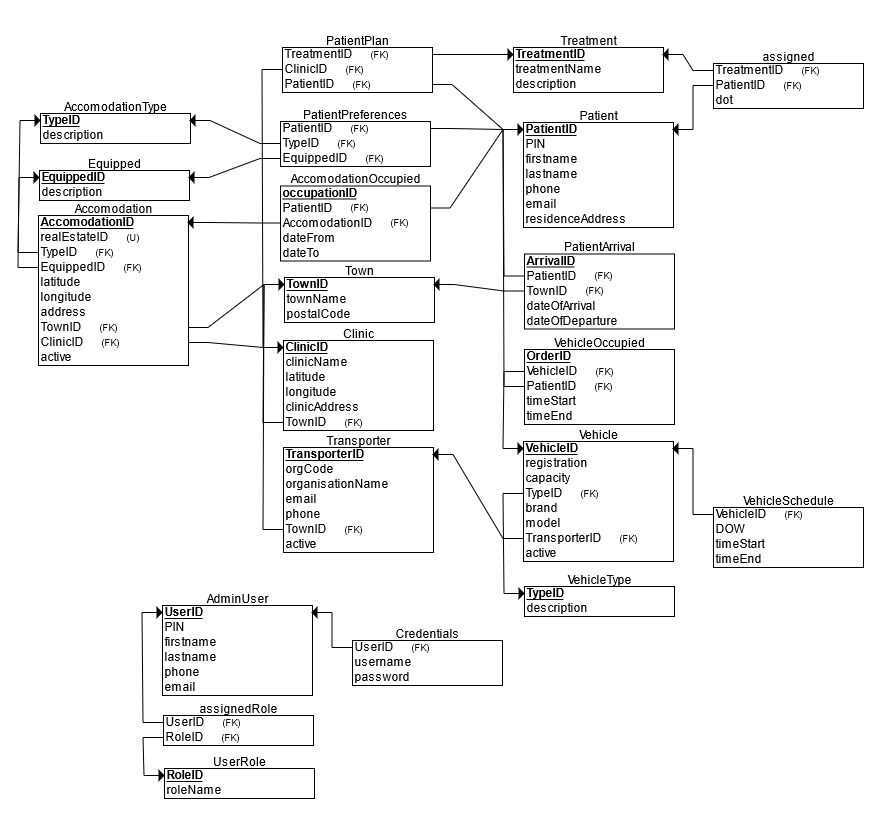
\includegraphics[width=\textwidth]{slike/DB_shema.PNG} %veličina u odnosu na širinu linije
					\caption{Sheme baze podataka}
					\label{fig:db_scheme} %label mora biti drugaciji za svaku sliku
				\end{figure}
			%Beskorisni komentar ....... :) MUAHHAHAHAH
			\eject
			
			
		\section{Dijagram razreda}
		
			Na slikama 4.2 i 4.3 su prikazani razredi \textit{Model} i \textit{Controller} iz MVC arhitekture. Razredi prikazani slikom 4.2 nasljeđuju razred Controller. Metode koje smo definirali unutar tih razreda pripremaju podatke i šalju ih bazi koja ih onda obrađuje. Baza manipulira modelima te na kraju vraća podatke kako bi ih \textit{View} mogao prikazati. Model razredi, prikazani slikom 4.3, prikazuju strukturu baze podataka te integrirane funkcije koje služe za obradu, slanje ili primanje podataka.
			
			\begin{figure}[H]
				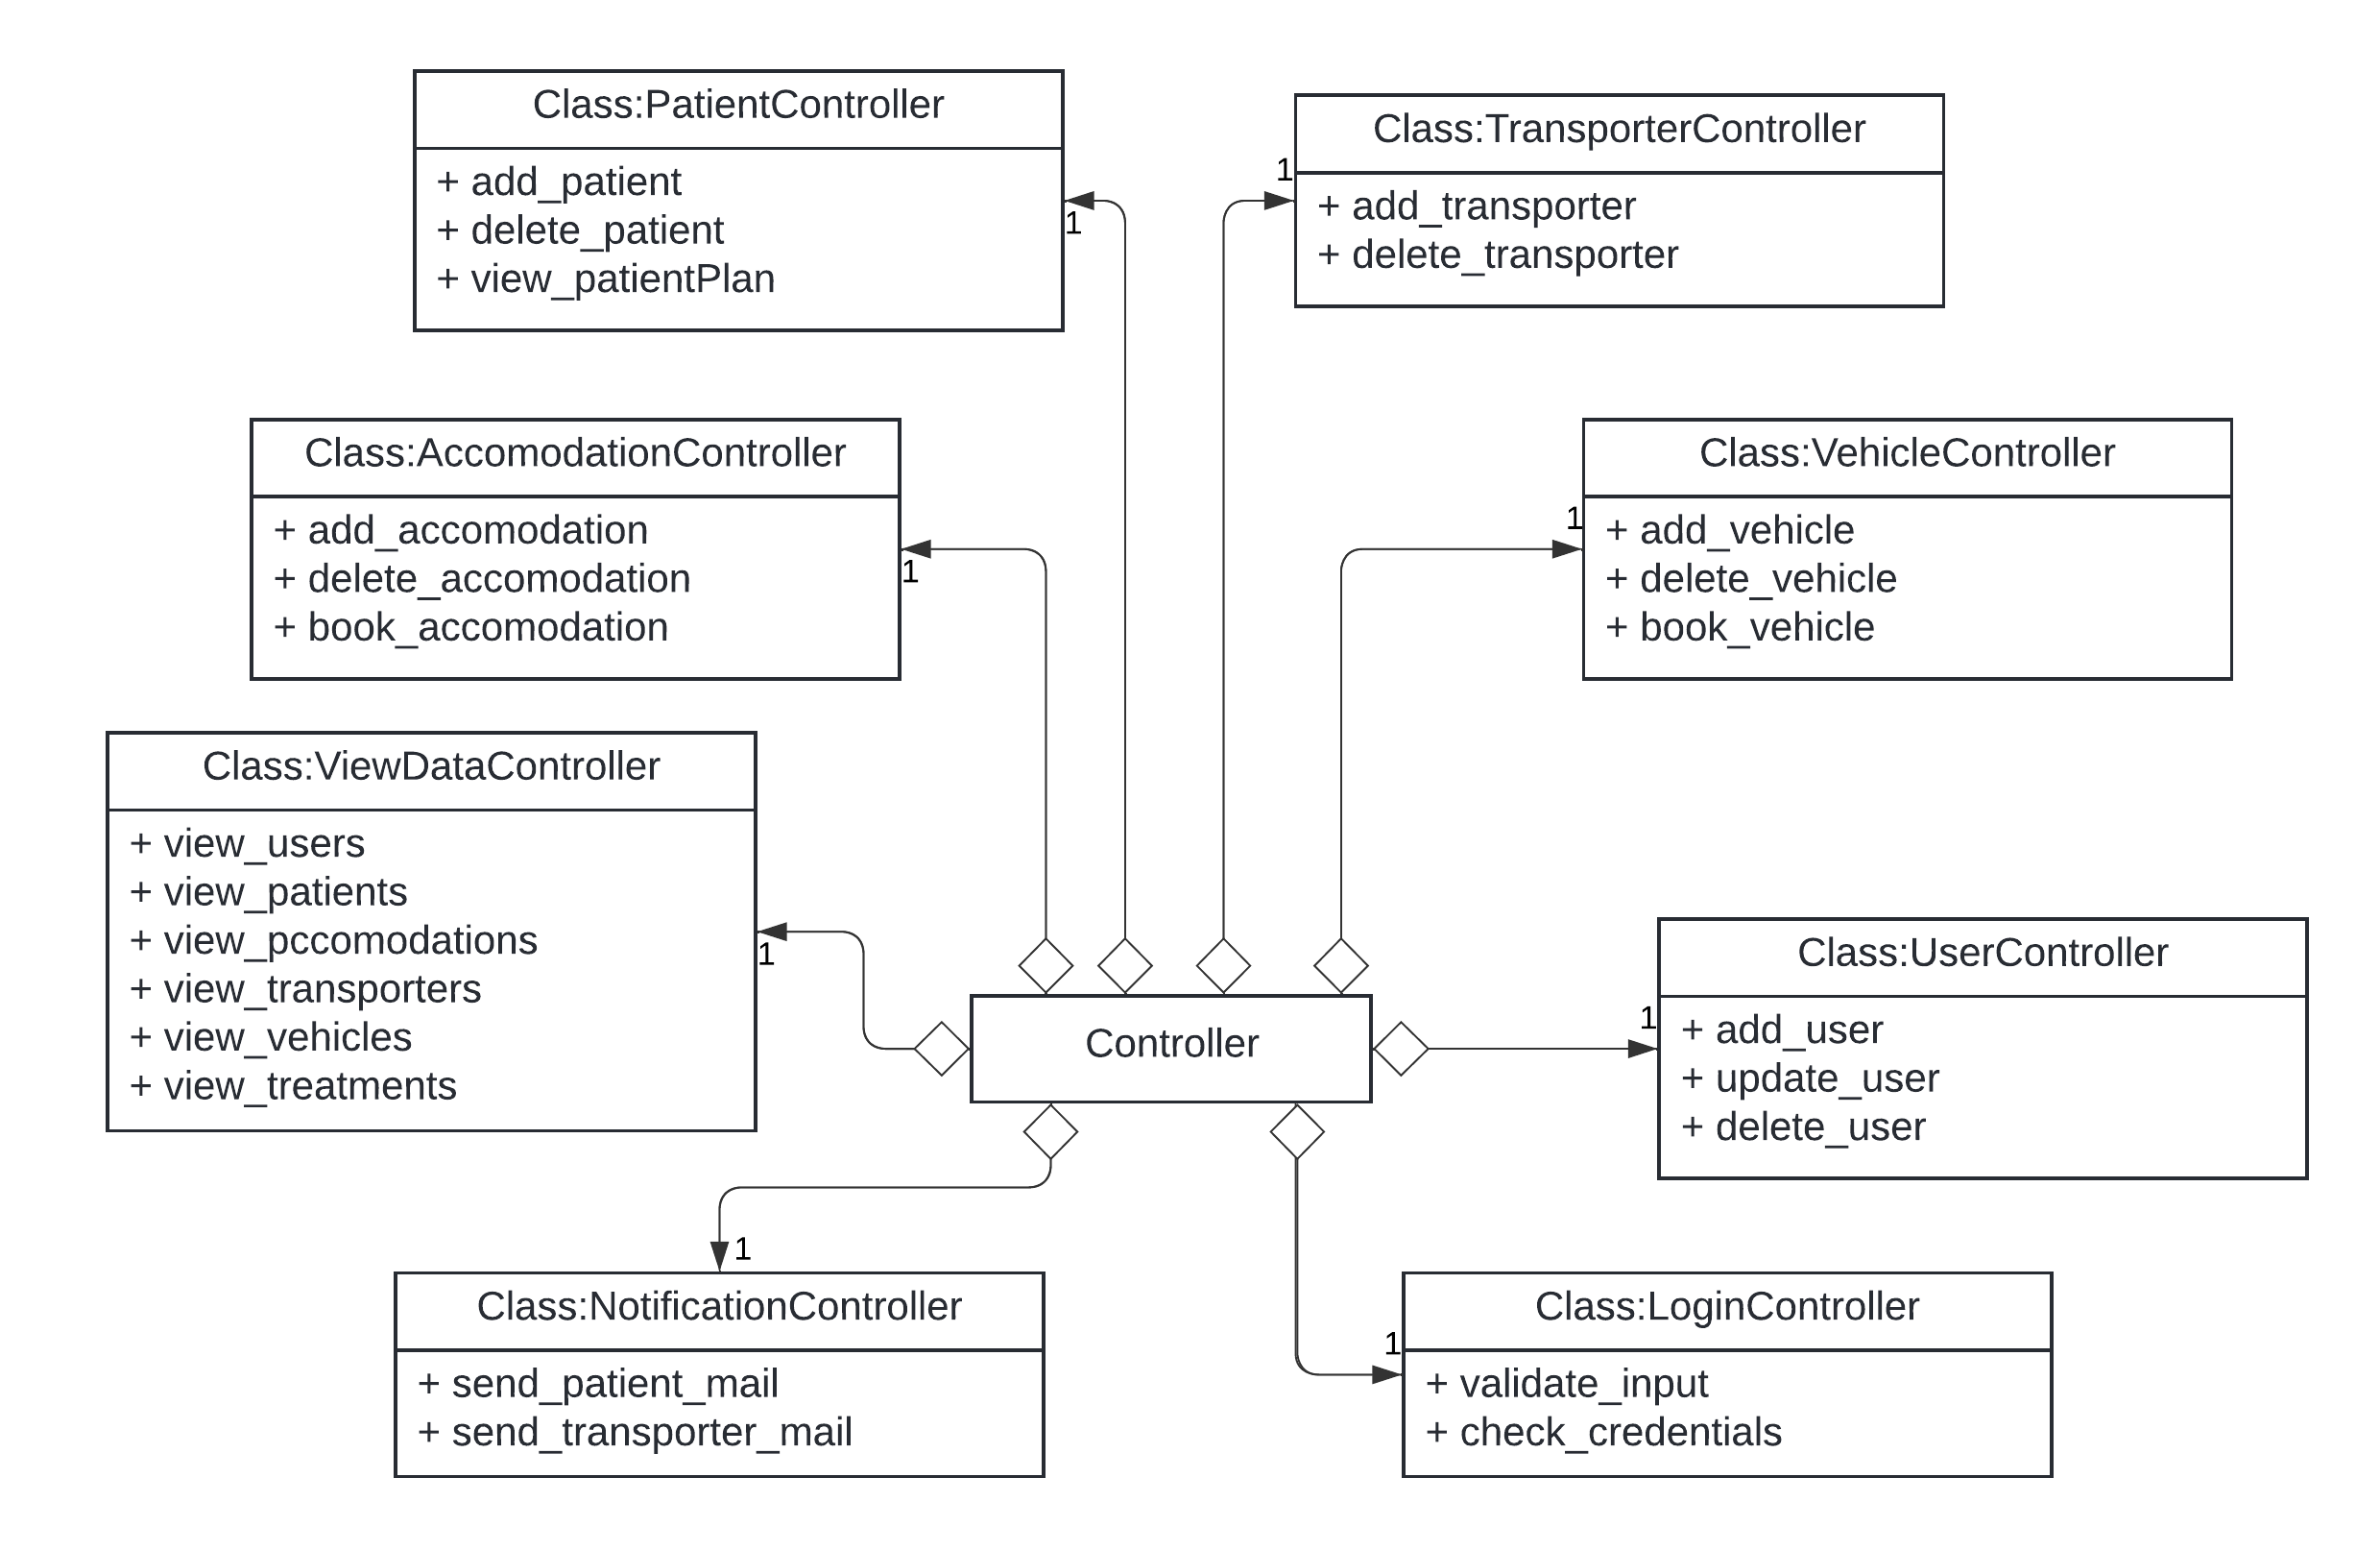
\includegraphics[width=\textwidth]{slike/UML_controller.PNG} %veličina u odnosu na širinu linije
				\caption{Dijagram razreda Controller}
				\label{fig:uml_controller} %label mora biti drugaciji za svaku sliku
			\end{figure}
			
			\begin{figure}[H]
				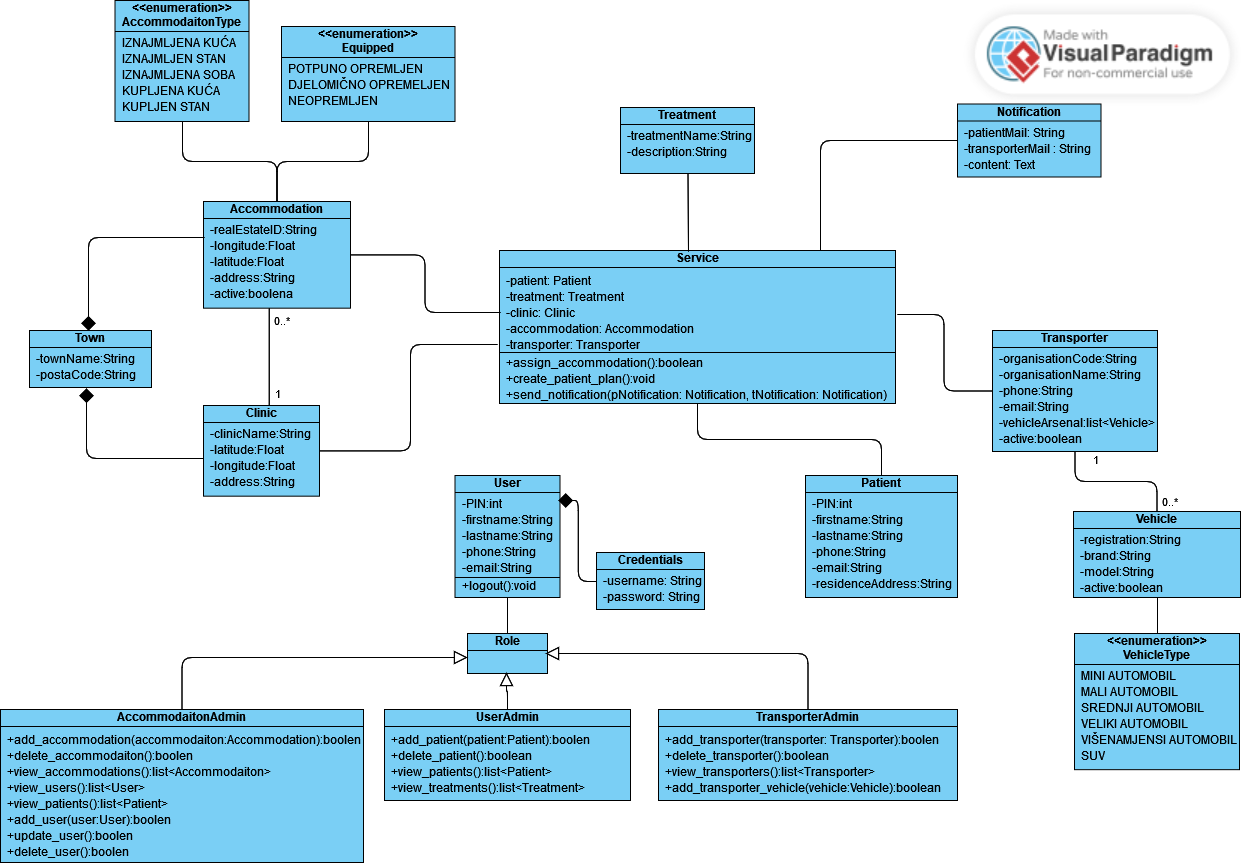
\includegraphics[width=\textwidth]{slike/UML_new_model.PNG} %veličina u odnosu na širinu linije
				\caption{Dijagram razreda Model}
				\label{fig:uml_model} %label mora biti drugaciji za svaku sliku
			\end{figure}
			\eject
		
		\section{Dijagram stanja}
			
			
			\textbf{\textit{dio 2. revizije}}\\
			
			\textit{Potrebno je priložiti dijagram stanja i opisati ga. Dovoljan je jedan dijagram stanja koji prikazuje \textbf{značajan dio funkcionalnosti} sustava. Na primjer, stanja korisničkog sučelja i tijek korištenja neke ključne funkcionalnosti jesu značajan dio sustava, a registracija i prijava nisu. }
			
			
			\eject 
		
		\section{Dijagram aktivnosti}
			Na slici 4.4 prikazan je dijagram aktivnosti. Prikazan je postupak periodičkog dodjeljivanja smještaja i prijevoza pacijentima. Korisnički administrator unosi podatke pacijenta, a sustav provjerava točnost podataka. Ako su podaci točni, sustav dodjeljuje dostupan smještaj, a ako smještaj nije dostupan, sustav periodički provjerava dostupnost dok ne nađe odgovarajući smještaj. Sličan proces se odvija i za prijevoz pacijenata - ako je prijevoz dostupan, sustav ga dodjeljuje; ako nije, sustav čeka i ponovno provjerava. Nakon uspješnog dodjeljivanja smještaja i prijevoza, podaci se ažuriraju u bazi podataka, a korisnički administrator se obavještava o uspješnom završetku procesa.
			\begin{figure}[H]
				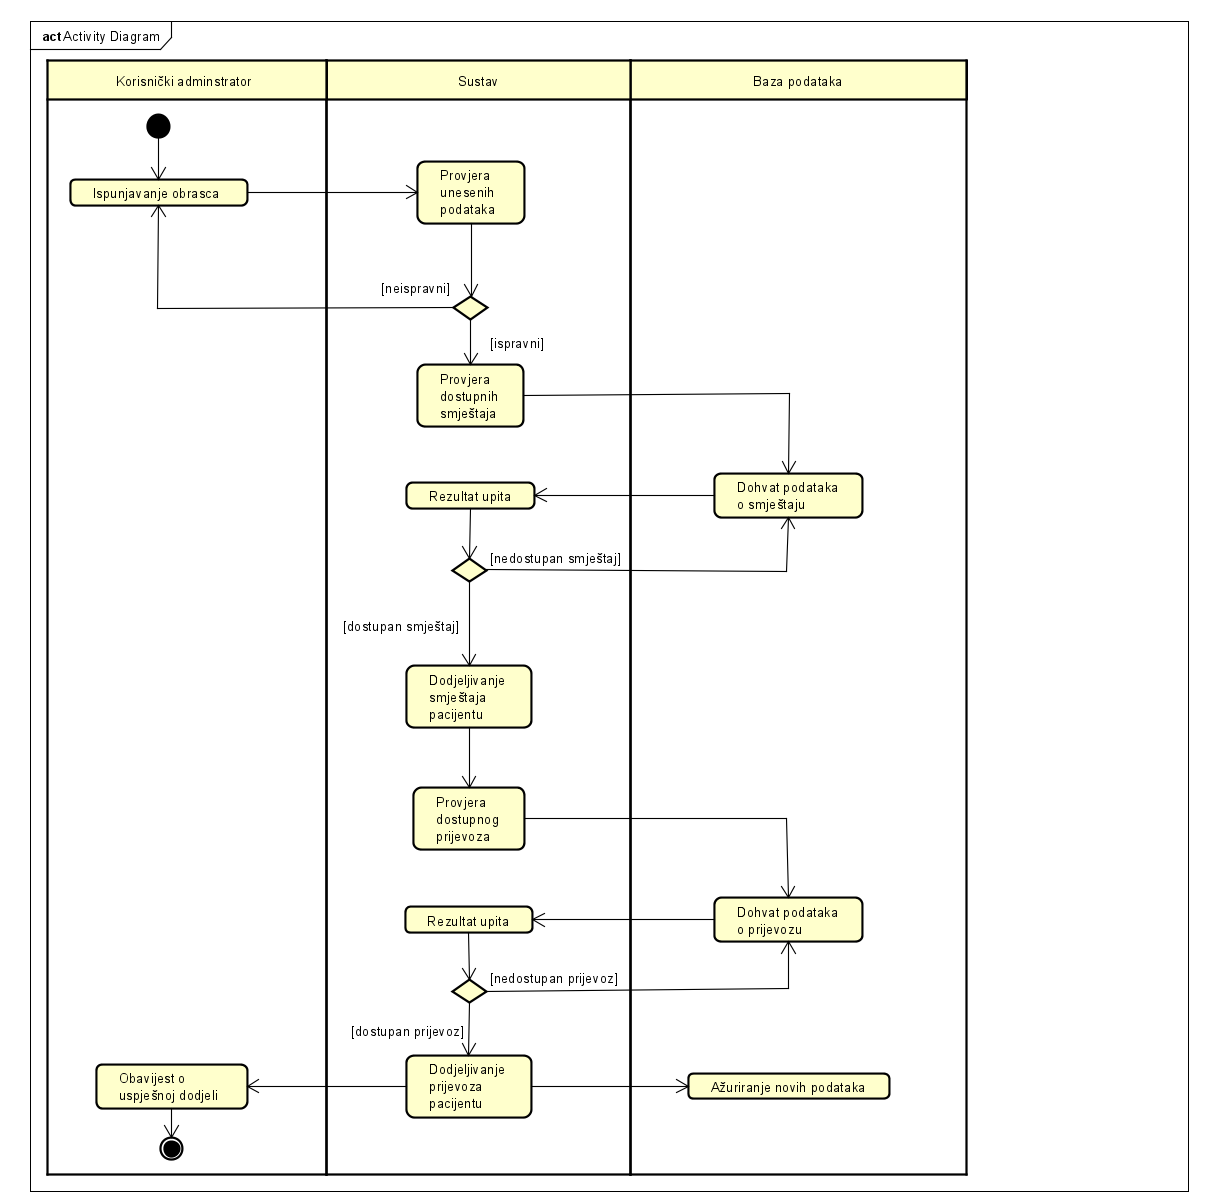
\includegraphics[width=\textwidth]{slike/UML_ActivityDiagram.png} %veličina u odnosu na širinu linije
				\caption{Dijagram aktivnosti}
				\label{fig:Dijagram aktivnosti} %label mora biti drugaciji za svaku sliku
			\end{figure}
			
			\eject
		\section{Dijagram komponenti}
		
			\textbf{\textit{dio 2. revizije}}\\
		
			 \textit{Potrebno je priložiti dijagram komponenti s pripadajućim opisom. Dijagram komponenti treba prikazivati strukturu cijele aplikacije.}